\documentclass{ieeeaccess}
\usepackage{cite}
\usepackage{amsmath,amssymb,amsfonts}
\usepackage{algorithmic}
\usepackage{graphicx}
\usepackage{textcomp}
\usepackage{multirow}
\usepackage{ulem}
\usepackage{hyperref}

\def\BibTeX{{\rm B\kern-.05em{\sc i\kern-.025em b}\kern-.08em
    T\kern-.1667em\lower.7ex\hbox{E}\kern-.125emX}}
\begin{document}
\history{Date of publication xxxx 00, 0000, date of current version xxxx 00, 0000.}
\doi{10.1109/ACCESS.2017.DOI}

\title{Unsupervised Semantic Mapping for Healthcare Data Storage Schema}

\author{ \uppercase{Fahad Ahmed Satti}\authorrefmark{1,2},
	\uppercase{Musarrat Hussain}\authorrefmark{1},
	\uppercase{Jamil Hussain}\authorrefmark{3},
	\uppercase{Syed Imran Ali}\authorrefmark{1}, % \IEEEmembership{} 
	\uppercase{Taqdir Ali}\authorrefmark{1},
	\uppercase{Hafiz Syed Muhammad Bilal}\authorrefmark{1,2},
	\uppercase{TaeChoong Chung}\authorrefmark{1},and  \uppercase {Sungyoung Lee}\authorrefmark{1}
	\IEEEmembership{Member, IEEE}}
\address[1]{Department of Computer Science and Engineering, Kyung Hee University, Seocheon-dong, Giheung-gu South Korea (e-mail: \{fahad.satti, musarrat.hussain, imran.ali, bilalrizvi, sylee\}@oslab.khu.ac.kr,  tcchung@khu.ac.kr)}
\address[2]{National Univeristy of Sciences and Technology, School of Electrical Engineering and Computer Science NUST-SEECS, Islamabad, Pakistan (e-mail: \{fahad.satti, bilal.ali\}@seecs.edu.pk)}
\address[3]{Department of Data Science, Sejong University, Seoul, South Korea (e-mail: jamil@sejong.ac.kr)}
\tfootnote{}



\markboth
{Fahad \headeretal:Unsupervised Semantic Mapping for Healthcare Data Stroage Schema}
{Fahad \headeretal:Unsupervised Semantic Mapping for Healthcare Data Stroage Schema}


\corresp{Corresponding authors: Sungyoung Lee (e-mail: sylee@oslab.khu.ac.kr) and TaeChoong Chung (e-mail: tcchung@khu.ac.kr)}

\begin{abstract}
Data, information, and knowledge processing systems, in the domain of healthcare, are currently plagued by heterogeneity at various levels. Current solutions have focused on developing a standard-based, manual intervention mechanism, which requires a large number of human resources and necessitates the realignment of existing systems. State-of-the-art methodologies in the field of natural language processing and machine learning can help to partially automate this process, reducing the resource requirements and providing a relatively good multi-class-based classification algorithm. We present a novel methodology for bridging the gap between various healthcare data management solutions by leveraging the strength of transformer-based machine learning models, to create mappings between the data elements. Additionally, the annotated data, collected against five medical schemas and labeled by four annotators is made available for helping future researchers. Our results indicate, that for biased, dependent multi-class text classification, transformer-based models provide better results than linguistic and other classical models. In particular, the Robustly Optimized BERT Pretraining Approach (RoBERTa) provides the best schema matching performance by achieving a Cohen's kappa score of 0.47 and Matthews Correlation Coefficient (MCC) score of 0.48, with human-annotated data.
\end{abstract}

\begin{keywords}
Context awareness, Decision support systems, Expert systems, Health information management, Medical information systems, Ontology engineering, Text processing, Unsupervised learning
\end{keywords}

\titlepgskip=-15pt

\maketitle

\section{Introduction}
\label{intro}
\PARstart{D}{ata} and Information modeling in the healthcare domain have witnessed significant improvements in the last decade owing to advances in the development of state-of-the-art Information and Communication Technologies (ICT) and formalization of storage and messaging standards. Subsequently, the scope of Healthcare Management Information Systems (HMIS), medical ontologies, and Clinical Decision Support Systems (CDSS) has broadened, beyond the operational capabilities of traditional rule based systems. One of the major reasons behind this limitation is due to the numerous heterogeneities in healthcare at data, knowledge, and process level. Thus, healthcare interoperability which aims to provide a solution to this problem, can be compartmentalized into data interoperability, process interoperability, and knowledge interoperability. Various abbreviations, used in this manuscript are listed in Table \ref{tab:abbreviations}.

Data interoperability resolves the heterogeneity between data artificats to enable seamless and interpretable communcation among source and target organizations, while preserving the data's original intention during storage, communication, and usage (as defined by IEEE 610.12 \cite{geraci1991ieee}, Health Level Seven International (HL7), and Healthcare Information and Management Systems Society HIMSS \cite{Himss_url2013}).
On the other hand, process interoperability regulates the communication among organizational processes to provide compatability between process artifacts within and seamless transformations across different organizations\cite{khan2013process}. Lastly, knowledge interoperability provides a sharing mechanism for reusing interpretable medical knowledge, acquired through expert intervention and other mechanisms, across decision support systems \cite{ali2017multi}.

\begin{table}[]
	\centering
	\caption{Abbreviations}
	\label{tab:abbreviations}
	\begin{tabular}{ll}
		\hline
		Abbreviations              & Full Form                                               \\ \hline
		ICT                        & Information and Communication Technologies              \\
		HMIS                       & Healthcare Management Information Systems               \\
		CDSS                       & Clinical Decision Support Systems                       \\
		HL7                        & Health Level Seven International                        \\
		HIMSS                      & Healthcare Information and Management Systems Society   \\
		FHIR                       & Fast Healthcare Interoperability Resources              \\
		Snomed-CT                  & Systematized Nomenclature of Medicine—Clinical Terms    \\
		LOINC                      & Logical Observation Identifiers Names and Codes         \\
		MLM                        & Medical Logic Module                                    \\
		openCIMI                       & Clinical Information Modeling Initiative                \\
		UHP                        & Ubiquitous Health Platform                              \\
		NLP                        & Natural Language Processing                             \\
		BERT                       & Bidirectional Encoder Representations from Transformers \\
		UMLS                       & Unified Medical Language System                         \\
		EMR 					   & Electronic Medical Records                              \\
		EHR						   & Electronic Health Records                               \\
		MCC                        & Matthews Correlation coefficient                        \\
		NLI                        & Natural Language Inference                              \\ \hline
	\end{tabular}
\end{table}

In more tangible terms, healthcare interoperability at data, process, and knowledge level can be exemplified within the healthcare constraints experienced due to the emergence of Covid 19. The operational capabilities of the current healthcare service delivery infrastructure has gone under tremendous stress due to Covid 19. World over, large primary healthcare units have managed to create separate units for managing patients, suffering from extreme cases of the novel coronavirus. For secondary and tertiary care units, government involvement has become necessary to filter coronavirus patients and adhering to a national pandemic response policy. 
These complex circumstances have enhanced the need for sharing patient data and state-of-the-art medical knowledge in real-time, to provide the medical experts with a tool to make accurate and timely decisions.
Data interoperability can enable the front line medical workers to fetch, understand, and use patient data, especially comorbidities, across organizational and physical boundaries, without suffering from societal taboos that may prevent the patient from sharing their complete and accurate medical histories. Knowledge interoperability can improve the knowledge acquisition and sharing protocols to provide the medical experts such as epidieomologists and vaccinologist, with latest information on affected population trends, disease diagnosis, treatment, and followup procedures, and interpretable decisions leading to positive or negative outcomes. Process interoperability can help reduce and in some cases remove the operational redundancies between health centers. In this way, successive healthcare treatments can take benefit from earlier diagnosis, treatment, and followup procedures, thereby reducing the stress on healthcare experts and systems. 
\\
Healthcare Standards such as HL7 - Fast Healthcare Interoperability Resources (FHIR), and openEHR provide the foundations for storing and communicating medical data, through the use of well defined protocols. While Systematized Nomenclature of Medicine—Clinical Terms (Snomed-CT) \cite{snomedct_url} and Logical Observation Identifiers Names and Codes (LOINC) \cite{loinc} provide a standard definition for clinical terminologies and laboratory tests, respectively. Similarly Medical Logic Module (MLM) provides a standardized way for expressing medical knowledge. Variety in these and many other healthcare standards necessitates the creation of bridging standards that can resolve the heterogeneity between the medical standards \cite{mohammed2010ubiquitous}. Substantial effort has gone into this endeavor with the Clinical Information Modeling Initiative (openCIMI) \cite{CIMI2015} taking the lead in bridging the gap between HL7v3 and openEHR. Similarly, SNOMED CT and LOINC are working to resolve the redundancies between the two terminological standards since 2013. This healthcare interoperability solution follows a formal, albeit long process, which is greatly dependent on the human factor. However, the current healthcare scenario requires a quick solution to create a scaffolding of an interoperable bridge between various healthcare providers. It is also important to ensure that this scaffolding should be able to support the formal standardization processes of the future. In \cite{Satti2020}, we have presented the Ubiquitous Health Platform (UHP), which provides semantic reconciliation-on-read based data curation for resolving data interoperability between various schema. This methodology is based on the creation and management of schema maps, that can provide the framework for transforming a source schema into a target schema. 
\\
In the current study, we will present our research work to build and manage the schema map knowledge base. Overall, our methodology is based on the creation, evaluation, and application of a novel schema matching technique to identify the relationships between attributes of the participating medical data schema. Since the terms used to identify attributes in the data schemas are not defined in any standard way, it is important to first identify the component words of the attribute term and then to append semantic concepts with these to create a meaningful sentence. This process is based on word expansion using concept lookup from Unified Medical Language System (UMLS). Once the sentence has been created, it is then trivial to create its embedded vectors representation using transformer based pre-trained models. The cosine similarity of any two embedded vectors can then indicate the degree of similarity between the original attributes. The motivation behind this methodology along with its development and evaluation details will be presented in the following flow:

\begin{itemize}
	\item[$-$] Section \ref{relatedwork} presents the related work
	\item[$-$] Section \ref{methodology} contains the details of our methodology
	\item[$-$] Section \ref{experimentalSetup} provides the experimental setup
	\item[$-$] Section \ref{results} presents the results
	\item[$-$] Section \ref{discussion} discusses the challenges and limitations of the presented methodology and its evaluations
	\item[$-$] Section \ref{conclusion} concludes the paper.
\end{itemize}



\section{Related Work}
\label{relatedwork}
Althubait et al. \cite{althubaiti2020combining} proposed an ontology expansion methodology that identifies and extracts new class from text articles using word embedding and machine learning techniques. The authors identified the similarity of tokens and phrases of the text articles with the exiting classes of the ontology. The target ontology is expanded with classes from text articles having greater similarity with that of already added classes. A similar word embedding technique was also used by Nozaki et al. \cite{nozaki2019semantic}, where the authors used instance based schema matching technique to identify the semantic similarity between two instances. The results of the study showed the possibility of detecting similar string attributes of different schemas. Yousfi et al. \cite{yousfi2020xmatcher} also utilized semantic base techniques and proposed xMatcher XML schemas matching approach. xMatcher transforms schemas into a set of words, followed by measuring words context, and relatedness score using WordNet. The terms from different schemas having similarities greater or equal to 0.8 are considered similar. 
Bylygin et al. \cite{bulygin2018combining} devised an ontology and schema matching approach by combining lexical and semantic similarity with machine learning approaches.  The authors used lexical and semantic measures as features and trained various machine learning algorithms including Naive Bayes, logistic regression, and gradient boosted tree. The result achieved showed that the combination of algorithms outperformed the single modal.

Martono et al. \cite{martono2017review} provided an overview of a linguistic approach for schema matching. The authors presented various linguistic methods to identify token strings in element names, followed by similarity evaluation between various schema. The process starts by normalizing the strings, which can be achieved via tokenization, generalization, elimination or semantic tagging. The normalized strings are then categorized based on their information relatedness. Elements belonging to the same categories are then compared with each other using two similarity measures, which include Lavenstein distance between words and Jaro-distance between 3-grams character sub-strings. Alwan et al. \cite{alwan2017survey} has summarized the techniques used in literature for schema matching based on database schemas and instances. These techniques can be categorized based on the type of information used for schema matching which includes  schema level, instance level, hybrid (schema and instances) and auxiliary (which can include information from external sources). Accordingly, most research is focused towards schema level and instance level approaches which can utilize syntactic techniques (such as n-gram, and/or regular expressions) and/or semantic techniques (such as Latent Semantic Analysis, WordNet/Thesaurus, and Google Similarity), to achieve data/information interoperability.  Kersloot et al. \cite{kersloot2020natural} performed a comprehensive systematic review to evaluate Natural Language Processing (NLP) algorithms used for clinical text mapping onto ontological concepts. The authors categorized the findings of various studies based on the use of NLP algorithms, data, validation and evaluation techniques, result presentation, and generalization of results. The authors revealed that over one-fourth of the NLP algorithms used were not evaluated and have no validation. The systems that claimed generalization, were self evaluated and having no external validation.  

Xu et al. \cite{xu2003discovering} presented a framework for discovering indirect links besides direct links among schema elements. The indirect matches were detected for relations such as union, composition, decomposition, selection, and boolean. The indirect links are useful to handle concepts merge, split, generalization, and specialization. The matching techniques utilized in the study considered terminological relationships (word synonym and hypernym), structural characteristics, data-value characteristics, and expected data values. The experimental results revealed framework effectiveness by achieving more than 90\% precision and recall for direct and indirect link matching. 

\begin{figure*}[t!]
	\centering
	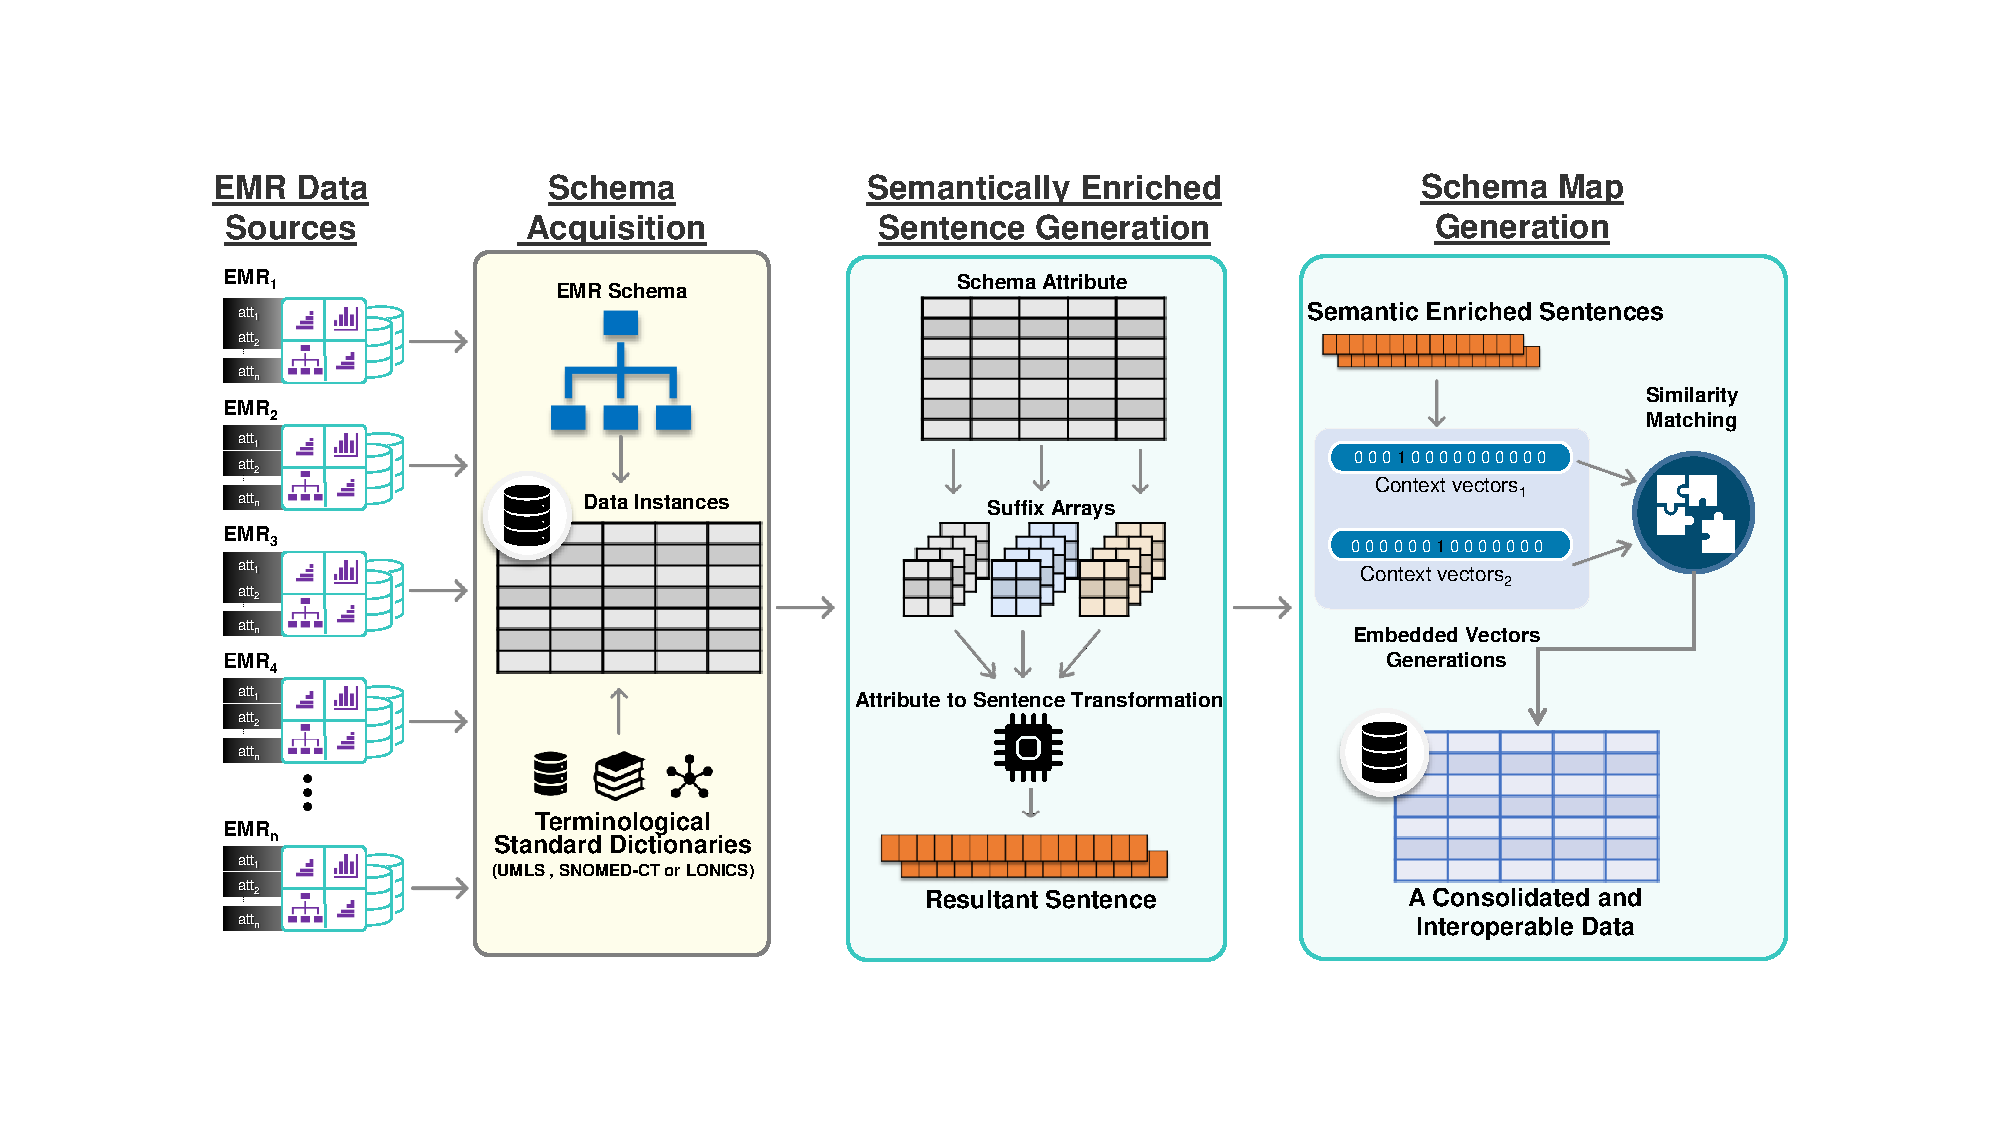
\includegraphics[scale=0.60]{methodology_final}
	\caption{Methodology for creating schema maps.}
	\label{fig:methodology}
\end{figure*} 

\section{Methodology}
\label{methodology}
Healthcare interoperability, with a focus on non-standard compliant medical schema is dependent on the generation and validation of schema maps as discussed above. To this end, the creation of a cohesive workflow is of utmost importance. In our earlier work \cite{Satti2020} we used maximum sequence identification and suffix trees based matching for syntactic matching of two distinct data schemas. This was followed by semantic concept enrichment and subsequently concept matching for creating rules in the form of schema maps. The simplified mapping functions, thereby created, provided a simple methodology for converting semi-structured medical data into an interpretable model form.
In our current methodology as visualized in Figure \ref{fig:methodology}, we have utilized state-of-the-art natural language processing (NLP) techniques to extract the schema mapping rules from semi-structured data schemas. This methodology is based on identifying similarity between vector representations of two attributes, belonging to different medical schemas. 
Traditional NLP techniques such as Word2Vec are able to convert a word into an embedded vector, while Bidirectional Encoder Representations from Transformers (BERT) extracts an embedded vector from a sentence \cite{zhu2018exploring}. Many of the attribute names within data schemas are represented by terms that are bigger than a word (combination of multiple words) and smaller than a sentence. In order to resolve this problem, we extracted the set of suffixes from the terms forming the attribute names. The bidirectional nature of BERT, allows the creation of contextual embedded vectors, where each target word is affected by its neighboring words. Hence to convert the set of suffixes into a sentence, we collected the set of concepts corresponding to each suffix, from UMLS. This operation has two effects, firstly it is used to remove any suffix, which does not have a corresponding concept and secondly the extracted concepts are used to add context to each suffix and produce a contextual sentence. 
The following subsections provide the practical details for our methodology from schema acquisition to attribute name expansion, and finally schema map generation.

\subsection{Schema acquisition}
\label{schema_acq}
In the first step of our semantic reconciliation methodology, we simulate medical data acquisition from five distinct Electronic Medical Records (EMR) storage systems ($S$). These include patient reports from OpenEMR ($s_1$), 100,000 patient records from EMRBOTS ($s_2$) \cite{kartoun2016methodology}, custom database design by Pan et. al($s_3$) for supporting regional clinics and health care centers in China \cite{pan2016design}, clinical knowledge discovery tool MedTAKMI-CDI ($s_4$) \cite{inokuchi2007medtakmi}, and our custom implementation ($s_5$) \cite{ali2017reconciliation}. Each of these medical systems as shown in Figure \ref{fig:schema}, follows the relational database design with logical entities such as demographics, diagnosis, medicine or others, placed into tables which can be further linked to one or more tables. While the database design implemented by each of these systems, fulfills the need of their respective information processing applications, the lack of interoperability, in terms of identifying similar attributes or exchanging the medical data is very much evident here. 


\begin{figure*}[t!]
	\centering
	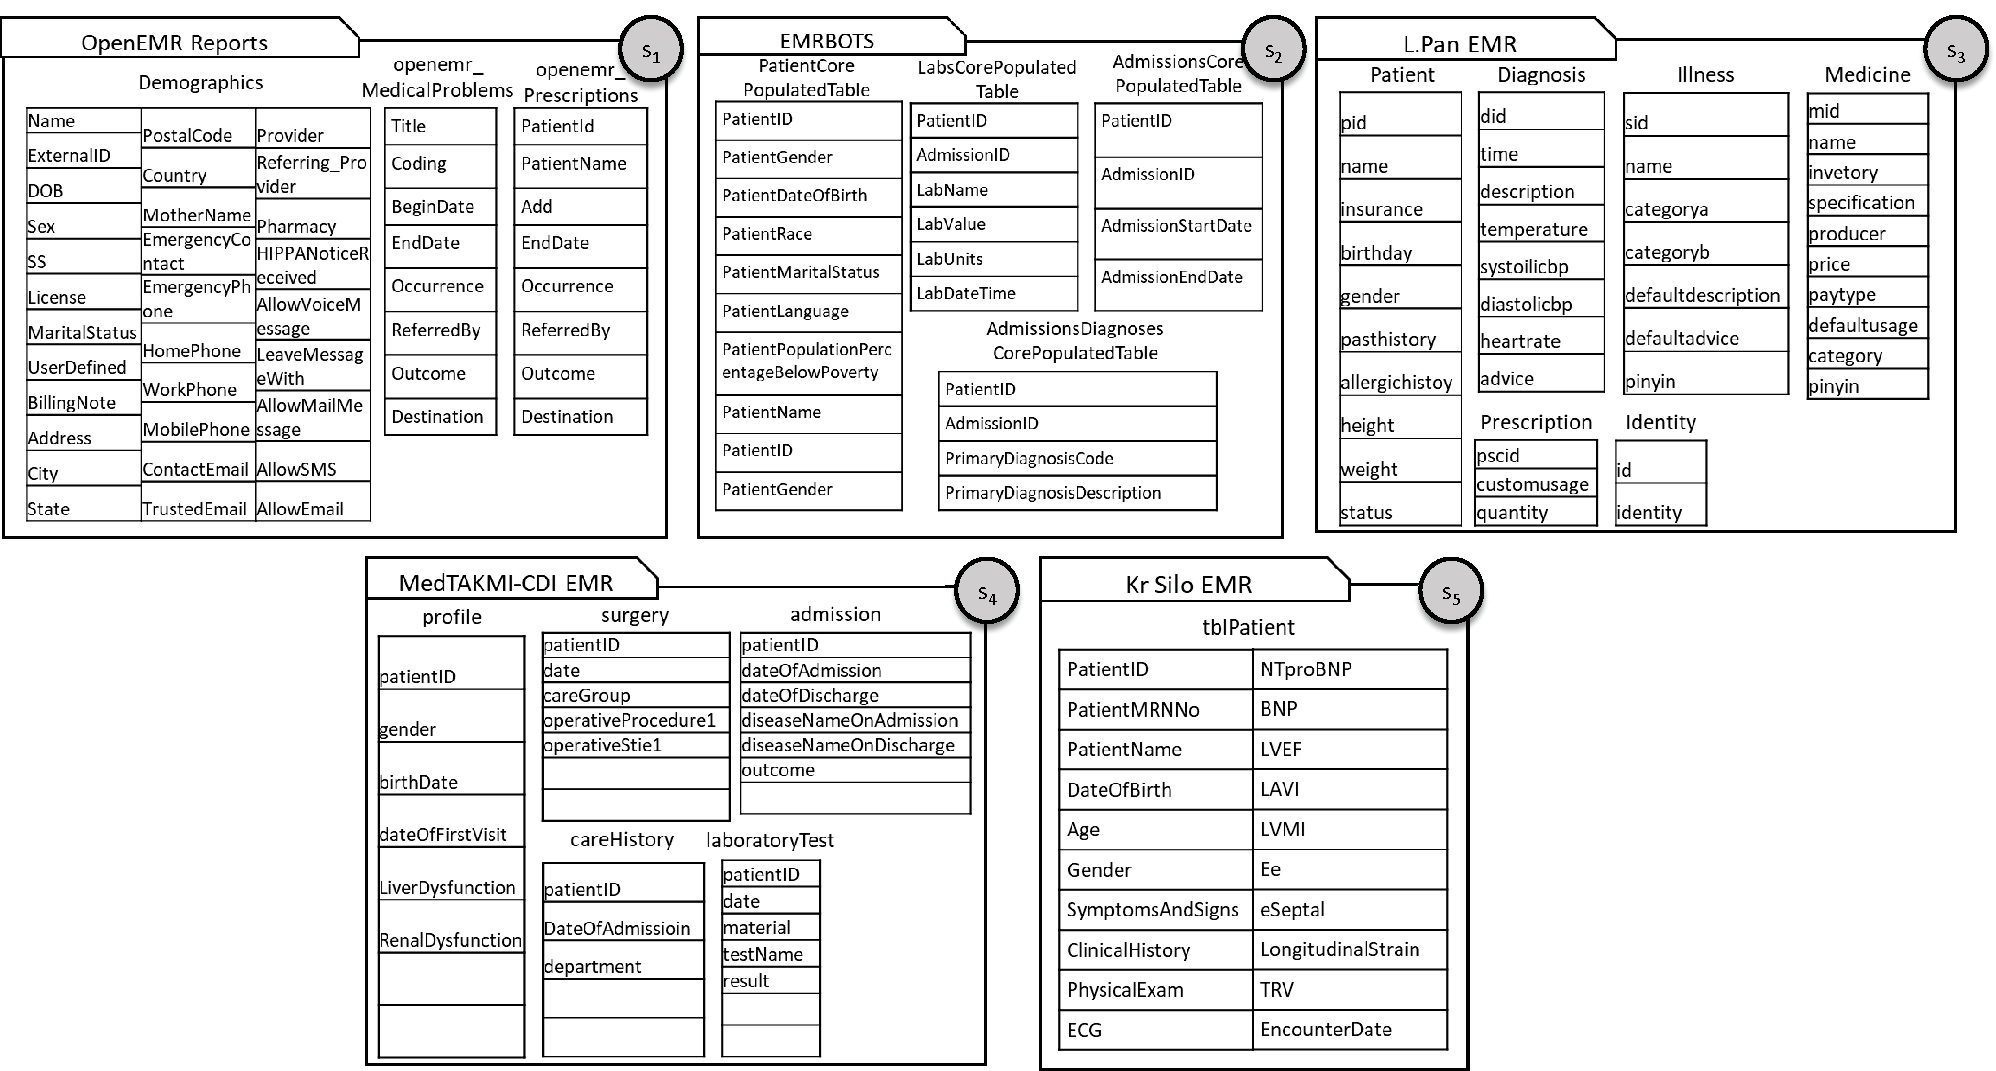
\includegraphics[scale=0.53]{schemas_final}
	\caption{The five medical schemas used for achieving data interoperability.}
	\label{fig:schema}
\end{figure*} 

A similar notion of data heterogeneity, in terms of medical data schema is evident across the healthcare domain. This is caused by various factors, including the lack of one all-encompassing, and universally applicable terminological standard and different normalization level for representing attributes.\\
In the former case, while SNOMED-CT provides a mechanism for identifying the standard codes for clinical terms and LOINC can be used for laboratory related terms, most attribute names are created based on the gut feeling of the database designer. Additionally, while these codes can be used to represent elements in the data instances (such as when recording the disease name, a standard code is more beneficial than the text string for semantic interoperability), the elements in a data schema (such as attribute names which are used in queries) achieve no benefit from the same.  Consider the terms ``name'' and ``patientName'', which refer to the same attribute of the patient entity.  However, since there is no standard way to represent this attribute, both are considered correct ($s_1$ and $s_3$ use the former representation, while $s_2$ and $s_5$ use the latter).\\
In the later case, differences in normalization cause semantic differences, due to which some data could be available in one schema but absent in others such as OpenEMR demographics identifying the patient's residential location using specific attributes like ``Address'', ``City'', ``State'', ``Postal Code'', ``Country'', and others. Similarly, ``EncounterDate'' from $s_5$ is semantically similar to ``BeginDate'' of ``openemr\_MedicalProblems'' table in $s_1$, ``AdmissionStartDate'' of ``LabsCorePopulatedTable'' in $s_2$, 
``time'' in ``Diagnosis'' table of $s_3$, and  ``dateOfAdmission'' in ``Diagnosis'' and ``CareHistory'' tables of $s_4$.
Finally, $s_1$ and $s_3$ have separate tables containing the medicinal prescription details, however the same details are unavailable in $s_2$, $s_4$, and $s_5$. Once again, this is not an incorrect behavior since this information, might not be a part of the context or the requirements for the EMR/EHR storage systems.
In fact, the change in context of the medical data storage system from the initial time of development to a later stage of collaborative processing systems, is the main cause of heterogeneity. In order to provide an interoperable solution, it is therefore necessary to enhance the semantics of each data attribute by its contextually equivalent sentence. 



\subsection{Attribute to Sentence Transformation}
\label{schema_prepro}
In order to process the EMR/EHR schema set $S$ and produce a set of corresponding semantically enriched sentences, we use the data representation $s_i$, generated through the process explained in sequence acquisition to collect the various medical fragments in memory. We then iterate over these fragments, building a set of attributes, distinguished by their name, schema's name, table's name, schema's version, source, and recorded data. This entails that ``PatientID'' from each of the four tables in $s_2$, and ``patientID'' from five tables in $s_4$, would result into nine attributes (assuming, as in the current case of no differences in versions of these systems).
For each attribute, we then generate the suffix array, which provides all possible substring representations contained within the attribute name. In order to generate the set of suffixes, we employ three strategies, forward suffix generation, whereby for a word $w$ of length $n$, $n-1$ suffixes of size 2 to $n-1$ are produced, backward suffix generation, to produce $n-1$ suffixes in reverse order with size $n-1$ to 2, and regular expression based suffix generation, which splits each word on, change of case, special characters(such as -, \_, !, and others), and numbers. In this way a large list of suffixes is generated, which is combined using a ``TreeSet'' data structure of Java, which internally sorts this list as well. An example of this suffix generation process, using the attribute name ``dateOfAdmission'' as it appears in $s_4$ is shown in Figure \ref{fig:suffix_attribute}.


\begin{figure}[tb!]
	\centering
	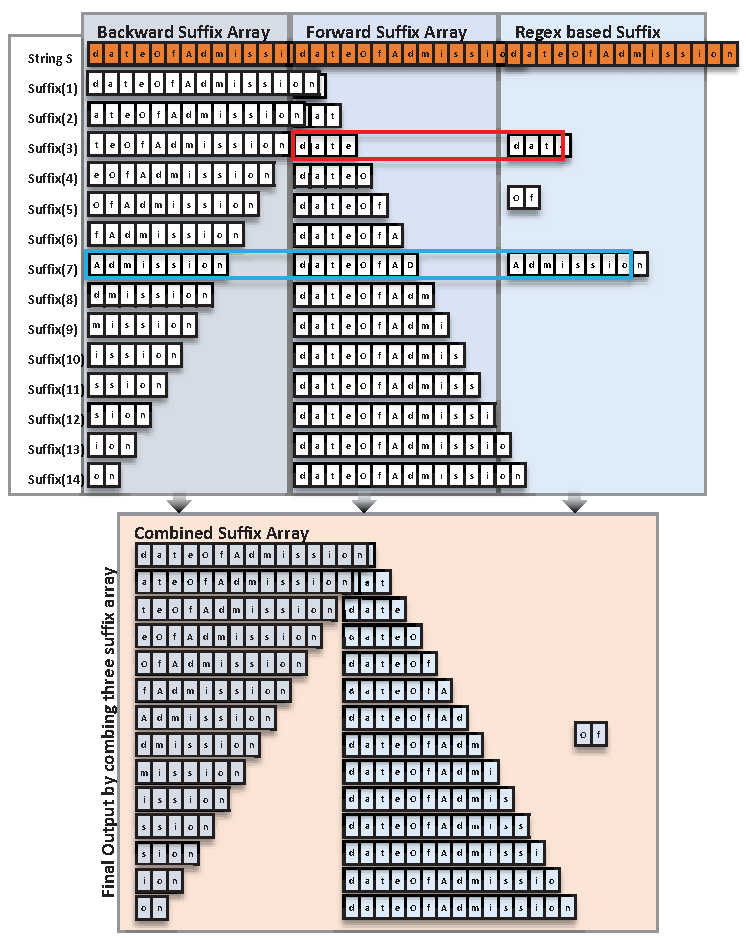
\includegraphics[scale=0.65]{suffixAttribute_final}
	\caption{An example of suffix arrays produced for the attribute ``dateOfAdmission''.}
	\label{fig:suffix_attribute}
\end{figure}


Suffix strings for similar attributes such as ``AdmissionStartDate''. ``diseaseNameOnAdmission'', and ``AdmissionEndDate'' appear in $s_2$, produce many, synctactically similar suffixes, to the presented example. This process, is only able to generate syntactic suffixes, producing many incoherent and unrelated suffixes. In order to counter this problem, and to limit the list of suffixes within the domain, we then query UMLS with exact search strategy, looking for the existence of any concepts against each suffix. In case, no semantic concept is found for a particular suffix, it is removed from the final Suffix Array. On the other hand, if atleast one semantic concept is found against the queried suffix, it is retained. Meanwhile the process continues for the next attribute, then the next table, and finally the next system, till no further processing is possible. 
The set of suffixes and their corresponding concepts are then used to build the sentence, where by each concept corresponding to a suffix is appended next to the suffix. An example of the resultant sentence for the attribute ``DateOfAdmission'' is shown in Table \ref{tab:sentence_example}.

\begin{table}[]
	\centering
	\caption{Sentence created from the attribute name ``DateOfAdmission''}
	\label{tab:sentence_example}
	\begin{tabular}{|p{\linewidth}|}
		\hline
		Date Value type - Date date allergenic extract Date in time Data types - Date Date Fruit;Of SPI1 wt Allele SPI1 gene TAF1 wt Allele BRIP1 gene Within Degrees fahrenheit Oral contraception BRIP1 wt Allele;Da Displacement of abomasum dalton Anterior descending branch of left coronary artery deca units cytarabine/daunorubicin protocol Dai Chinese Asymptomatic diagnosis of Drug Accountability Domain;ion Iontophoresis Route of Drug Administration Ions;on SPARC wt Allele Osteonectin SPARC gene On (qualifier value) Upon - dosing instruction fragment;Admission Admission activity Hospital admission;Dat SLC6A3 gene SLC6A3 wt Allele dopamine transporter Direct Coombs test SLC6A3 protein, human Test Date cytarabine/daunorubicin/thioguanine Alzheimer's Disease;mission Religious Missions;\\
		\hline
	\end{tabular}
\end{table}

Here the various suffixes and their concepts are separated by the symbol ``;'', however together they form one sentence, for which an embedded vector is generated. 

\subsection{Schema Map generation}
\label{schema_map_gen}

Schema Maps provide an interoperable bridge between two medical systems ($s_i \wedge s_j$), by identifying the semantic relationship between their participating attributes. This identification is based on the similarity between the embedded vectors, of the semantically enriched sentences corresponding to each data attribute. While the embedded vectors can be generated using any methodology, we tested 11 methodologies with Word2Vec and 10 models based on BERT further detailed in section \ref{experimentalSetup}. Our results indicate that the large/STSb version of Robustly Optimized BERT Pretraining Approach (RoBERTa)\cite{reimers-2019-sentence-bert}, provides the best matching results. The pair of embedded vectors thus produced are then used to calculate cosine similarity, which is based on the inverse cosine distance between them. For our classification, we used the raw results (unnormalized) of cosine similarity, which produces a score between -1, and 1. Cosine similarity score of 0 indicates orthogonal relationship between the two vectors, which in our scenario indicates that the two sentences, and by extension their attributes are not related to each other. -1 indicates inverse relationship between the attributes, while 1 indicates the two attributes are very much the same.
For producing our schema maps, we are interested in three types of relationships, ``equal'' (the two attributes are same), ``related'' (the two attributes are related to each other), and ``unrelated'' (no relationship between the attributes). In order to classify the similarity results into one of these three classes, we then calculated the best thresholds using Matthews Correlation coefficient (MCC) \cite{chicco2020advantages} for classifying each instance as ``equal'', ``related'', and ``unrelated''. 

\begin{equation}
\label{eq:mccformula}
\resizebox{0.9\hsize}{!}{$%
	MCC = \frac{(TP \times TN) - (FP \times FN)}{\sqrt{(TP+FP)\times(TP+FN)\times(TN+FP)\times(TN+FN)}}\longrightarrow [-1,1]
	$%
}%
\end{equation}
MCC provides a fair measure of the ability with which a classifier can correctly predict both positive and negative instances \cite{chicco2020advantages}. The formula for calculating MCC is shown in Equation \ref{eq:mccformula}, which is based on classification performance measures such as true positive (TP), true negative (TN), false positive (FP), and false negative (FN). MCC score of 0 represents random classification, however, with an increase in the number of true positives and true negatives MCC moves closer to 1. It also takes into account the false positives and false negatives, which shift the MCC score towards -1. This measurement is markedly different from accuracy that fails to account for imbalanced datasets and $F_1$ measure which is not affected by the true negative scores. As a result, MCC provides an acceptable alternate in our current scenario comprising of imbalanced dataset (largely in favour of class ``unrelated'') to measuring the true performance of the models, used for threshold selection and model evaluation. Finally on a test dataset we evaluated our multi-class classification approach using MCC and Cohen's Kappa coefficient ($\kappa$) \cite{gwet2014handbook} to identify the relationships between each pair of attributes.

\section{Experimental Setup}
\label{experimentalSetup}
In our earlier work \cite{Satti2020} $s_1$, $s_2$, and $s_5$ were used to generate over 115 million patient records, which are converted into a semi-structured form and stored in Hadoop Distributed File System (HDFS). We extended the same setup to create an additional 100,000 records, for 1000 patients with 3 medical fragments for $s_1$, $s_2$, and $s_4$, and 97 randomly selected and generated medical fragments amongst $s_1$, $s_2$, $s_3$, $s_4$ and $s_5$. These fragments follow various design elements supporting a variety of valid relational storage architectures. Such as, $s_1$, $s_2$ and $s_4$ are represented by creating a separate medical fragment for each participating table, $s_3$ utilizes its medical fragment to generate a linked record (from a linked object graph), where by the attributes can refer to other objects, mimicking the application of explicit foreign keys, and $s_5$ is a flat table structure. The code to generate this data set is available at ``uhp\_map\_generation''\footnote{https://github.com/desertzebra/UHP\_v4/tree/main/uhpr\_storage}. This application produces three custom formatted files containing an index for patients, an index for their medical fragments, and the medical fragment corresponding to the EMR data. Using the medical fragments file, we then generate the semantically enriched attribute \footnote{https://github.com/desertzebra/UHP\_v4/tree/main/uhp\_map\_generation}, which contains the suffixes and their concepts corresponding to each EMR data attribute. The resulting set of enriched attributes are temporarily stored in a JSON file, which is then read by the same application to partially generate the schema maps. This process is used to create 20,349 distinct pairs of attributes across $s$. Each pair also contains the ``relationshipList'', which stores the results of fuzzy string matching\cite{FuzzyWuzzy} \footnote{Java Library: https://github.com/xdrop/fuzzywuzzy} between the attribute names. 
The JSON file thus produced is then used by a python script to generate the semantically enriched sentences and their embedded vectors using Word2Vec, and 10 pre-trained BERT NLI models \cite{reimers-2019-sentence-bert}. The BERT models include ``bert-base-nli-stsb-mean-tokens'', ``bert-large-nli-stsb-mean-tokens'', ``roberta-base-nli-stsb-mean-tokens'', ``roberta-large-nli-stsb-mean-tokens'', ``distilbert-base-nli-stsb-mean-tokens'', ``bert-base-nli-mean-tokens'', ``bert-large-nli-mean-tokens'', ``roberta-base-nli-mean-tokens'', ``roberta-large-nli-mean-tokens'', and ``distilbert-base-nli-mean-tokens''. 
The embedding vectors are then compared using cosine similarity. The rationale behind switching the applications at various stages is to cache the results and create checkpoints for restarting any failed stages, easily. Additionally, since python provides better support for easy generation of embedding vectors, it was thus preferred over the Java based implementation, which is otherwise very beneficial for other tools.
%These applications were executed on a workstation running Ubuntu 20.04.2 on top of AMD Ryzen 3 2200G, and 32GB ram.%

\section{Results}
\label{results}

The validity of our proposed approach has been evaluated using several techniques including comparison of the proposed semantic matching process with fuzzy string matching, embedded vector generation and comparison using Word2Vec, and 10 BERT nli models. 

\begin{figure}[htb!]
	\centering
	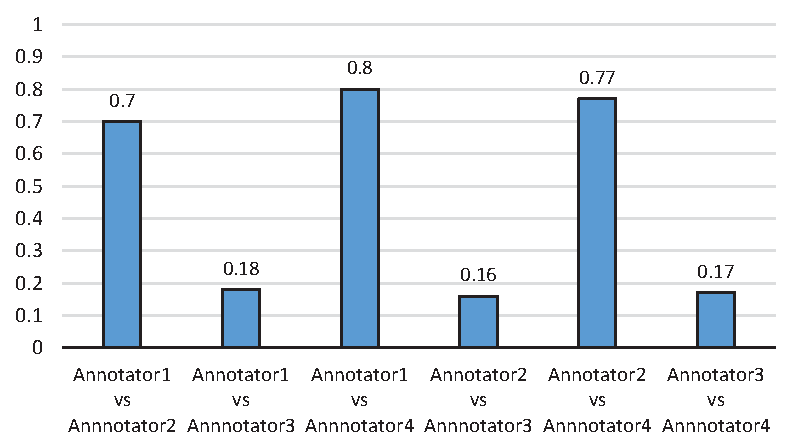
\includegraphics[width=\columnwidth]{kappaInterAnnotatorAgrement_final}
	\caption{Cohen's Kappa ($\kappa$) score among the four annotators}
	\label{fig:kappaInterAnnotatorAgrement}
\end{figure}

\subsection{Dataset Annotation}
In order to compare our computed models with ground truth and to identify the best thresholds for classifying each instance as ``equal'', ``related'', or ``unrelated'' four human annotators were utilized to anonymously, score the similarity of each pair of attribute names. In order to support this process, we first repurposed one of our generated data matrix by marking all attribute pairs belonging to the same schema with the symbol ``-''. Following this, the annotators marked each cell corresponding to a pair of attributes (conversely, each attribute pair corresponds to two cells with the positioning of the pair-participants swapped; which is used for clarity and identify correct relationships between the attribute on left and attribute on right), by determining the similarity in terms of dissimilar as ``0'', exactly similar as ``1'', row attribute as child of column attribute as ``<'', row attribute as a parent of the column attribute as ``>'', and finally, unknown as ``~''. The data sheets generated after this extensive human effort have been made available for other researchers\footnote{\url{https://github.com/desertzebra/EMR-Interoperability/tree/master/Implemenation/Data/Annotated}}.

\begin{table*}
	\centering
	\caption{Annotations performed by the four annotators on five medical schema}
	\label{tab:annotator_marking}
	\begin{tabular}{|l|l|l|l|l|l|}
		\hline
		Method     & Total Matches & Marked as Equal & Marked as Related & Marked as Unrelated & Not Marked \\ \hline
		Annotator1 & 40698         & 238             & 109               & 40351               & 0          \\
		Annotator2 & 40698         & 241             & 116               & 40341               & 0          \\
		Annotator3 & 40698         & 260             & 2103              & 38182               & 153        \\
		Annotator4 & 40698         & 225             & 62                & 40400               & 11         \\ \hline
	\end{tabular}
\end{table*}

These sheets, additionally contain some missing values, which were left out by the annotators but in order to maintain their originality, these values were not filled; instead during our evaluation for these datasets, the missing values were considered as having the score ``0''. Using $\kappa$, we evaluated the inter-rater agreement of these annotations, which have been visualized in Figure \ref{fig:kappaInterAnnotatorAgrement}. It can be seen in this plot, that ``Annotator3'' has very small correlation with the other 3 annotators. This difference can be traced back to the number and type of annotations performed by each annotator, which is shown in Table \ref{tab:annotator_marking}. The ``Annotator3'' has marked 2103 cells as related (one of >, < , or ~) and left 153 as empty. Even in the presence of these differences, it is pertinent to include the data for all annotators in order to avoid any bias. 

This annotated data was then processed to replace all related entries with ``0.5'' ($class_{0.5}$) and all ``-'' with ``0'' ($class_{0}$), while the values for similar at ``1'' ($class_{1}$) and ``0'' ($class_{0}$) for dissimilar were kept the same. This conversion was then used to produce a consolidated dataset of 40,698 attribute pairs using mode scores of all annotators for each cell. We also tested average scores between the annotators, but that would produce scores between ``0'', ``0.5'', and ``1'', greatly increasing the number of classes for classification. Hence the maximum agreement between the annotators maintains the final label values within these three classes, which become easier to evaluate. Additionally, the original dataset and its mode consolidated form is biased in favour of class ''0'', since most attribute pairs are not related to each other.
This dataset is then split into development and testing partitions with a ratio of 70:30. The development partition is used for threshold selection based on the best MCC score for identifying class ``equal'', followed by best scores for class ``related'' and finally best of class ''unrelated''. The optimal threshold thus achieved is used to classify the instances of the test dataset, which is finally evaluated on its MCC and $F_1$ measure.

\begin{figure*}[t!]
	\centering
	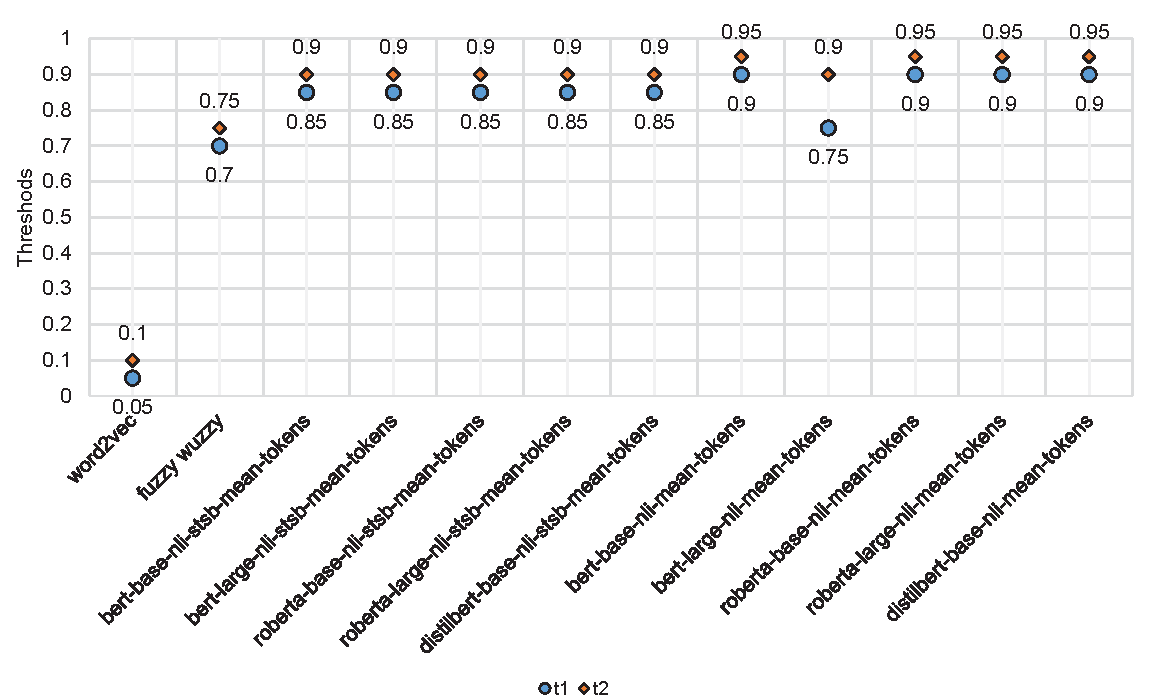
\includegraphics[scale=0.83]{thresholdSelection_final}
	\caption{Thresholds selection using MCC scores where t1 indicates the similarity threshold between $class_0$ and $class_{0.5}$, and t2 indicate the similarity threshold between $class_{0.5}$ and $class_1$.}
	\label{fig:thresholdSelection}
\end{figure*}

\subsection{Threshold Selection}
A good text classification methodology is dependent on the correct choice of a threshold, which can maximize the target class participation. In case of independent labels, area under the precision recall curve can provide this optimal measure, however as in our case, for dependent classes on a biased dataset the MCC, is better\cite{chicco2020advantages}.
Since our aim is to apply an optimal text similarity classifier to resolve this multi-class problem ($class_0$, $class_{0.5}$, and $class_1$), we have to test various threshold scores for separating the instances between $class_0$ and $class_{0.5}$ ($t_1$), and then $class_{0.5}$ and $class_1$ ($t_2$). Additionally, since our aim is to correctly identify the similar attribute instances, it is pertinent to maximize the classification performance of $class_1$ (similar), followed by $class_{0.5}$ (related), and finally $class_0$ (unrelated).
With a step size of \textit{0.05} ($step$), and starting from $t_1$ as 0.0 and $t_2$ as $t_1$ + $step$, we move the thresholds until $t_2$ reaches \textit{1.0}, followed by increase in $t_1$ by step size. Eventually, $t_1$, reaches \textit{0.95} and $t_2$ reaches \textit{1.0}, at which point, the process stops. This is to ensure that $t_1$ remains behind $t_2$, for all iterations, measuring MCC score, for the 12 models. These models include, ``Fuzzy\_Wuzzy'', ``Word2Vec'', and 10 BERT based models. The optimal thresholds achieved by each of these models is shown in Figure \ref{fig:thresholdSelection}.

% Please add the following required packages to your document preamble:
% \usepackage{multirow}
\begin{table*}[h!]
	\centering
	\caption{Performance matrix for individual classes using one vs all binarization technique}
	\label{tab:evaluations}
	\begin{tabular}{|c|c|c|l|l|l|l|l|}
		\hline
		\textbf{Model}                                        & \textbf{Class Positive} & \textbf{Class Negative} & \multicolumn{1}{c|}{\textbf{Accuracy}} & \multicolumn{1}{c|}{\textbf{Precision}} & \multicolumn{1}{c|}{\textbf{Recall}} & \multicolumn{1}{c|}{\textbf{F-1}} & \multicolumn{1}{c|}{\textbf{MCC}} \\ \hline
		\multirow{3}{*}{FUZZY\_MATCH}                         & $class_0$                     & $class_{0.5}$,$class_1$                   & 0.98                                   & 1.00                                    & 0.99                                 & 0.99                              & 0.37                              \\ \cline{2-8} 
		& $class_{0.5}$                     & $class_0$,$class_1$                   & 1.00                                   & 0.00                                    & 0.00                                 & 0.00                              & 0.00                              \\ \cline{2-8} 
		& $class_1$                       & $class_0$,$class_{0.5}$                 & 0.98                                   & 0.20                                    & 0.59                                 & 0.29                              & 0.33                              \\ \hline
		\multirow{3}{*}{Word2Vec}                             & $class_0$                     & $class_{0.5}$,$class_1$                   & 0.24                                   & 0.99                                    & 0.24                                 & 0.38                              & 0.01                              \\ \cline{2-8} 
		& $class_{0.5}$                     & $class_0$,$class_1$                   & 1.00                                   & 0.15                                    & 0.10                                 & 0.12                              & 0.12                              \\ \cline{2-8} 
		& $class_1$                       & $class_0$,$class_{0.5}$                 & 0.35                                   & 0.01                                    & \textbf{0.84}                        & 0.01                              & 0.03                              \\ \hline
		\multirow{3}{*}{bert-base-nli-stsb-mean-tokens}       & $class_0$                     & $class_{0.5}$,$class_1$                   & 0.99                                   & 1.00                                    & 0.99                                 & 0.99                              & 0.37                              \\ \cline{2-8} 
		& $class_{0.5}$                     & $class_0$,$class_1$                   & 1.00                                   & 0.00                                    & 0.00                                 & 0.00                              & 0.00                              \\ \cline{2-8} 
		& $class_1$                       & $class_0$,$class_{0.5}$                 & 0.99                                   & 0.22                                    & 0.50                                 & 0.30                              & 0.32                              \\ \hline
		\multirow{3}{*}{bert-large-nli-stsb-mean-tokens}      & $class_0$                     & $class_{0.5}$,$class_1$                   & 0.99                                   & 1.00                                    & 1.00                                 & 1.00                              & 0.51                              \\ \cline{2-8} 
		& $class_{0.5}$                     & $class_0$,$class_1$                   & 1.00                                   & 0.00                                    & 0.00                                 & 0.00                              & 0.00                              \\ \cline{2-8} 
		& $class_1$                       & $class_0$,$class_{0.5}$                 & 0.99                                   & 0.41                                    & 0.50                                 & 0.45                              & 0.45                              \\ \hline
		\multirow{3}{*}{roberta-base-nli-stsb-mean-tokens}    & $class_0$                    & $class_{0.5}$,$class_1$                   & 0.99                                   & 1.00                                    & 0.99                                 & 1.00                              & 0.40                              \\ \cline{2-8} 
		& $class_{0.5}$                     & $class_0$,$class_1$                   & 1.00                                   & 0.00                                    & 0.00                                 & 0.00                              & 0.00                              \\ \cline{2-8} 
		& $class_1$                       & $class_0$,$class_{0.5}$                & 0.99                                   & 0.26                                    & 0.50                                 & 0.34                              & 0.36                              \\ \hline
		\multirow{3}{*}{roberta-large-nli-stsb-mean-tokens}   & $class_0$                     & $class_{0.5}$,$class_1$                   & 1.00                                   & 1.00                                    & 1.00                                 & 1.00                              & 0.61                              \\ \cline{2-8} 
		& $class_{0.5}$                     & $class_0$,$class_1$                   & 1.00                                   & 0.00                                    & 0.00                                 & 0.00                              & 0.00                              \\ \cline{2-8} 
		& $class_1$                       & $class_0$,$class_{0.5}$                & \textbf{1.00}                          & \textbf{0.59}                           & 0.50                                 & \textbf{0.54}                     & \textbf{0.54}                     \\ \hline
		\multirow{3}{*}{distilbert-base-nli-stsb-mean-tokens} & $class_0$                     & $class_{0.5}$,$class_1$                   & 0.99                                   & 1.00                                    & 0.99                                 & 0.99                              & 0.38                              \\ \cline{2-8} 
		& $class_{0.5}$                     & $class_0$,$class_1$                   & 1.00                                   & 0.00                                    & 0.00                                 & 0.00                              & 0.00                              \\ \cline{2-8} 
		& $class_1$                       & $class_0$,$class_{0.5}$                 & 0.99                                   & 0.23                                    & 0.50                                 & 0.32                              & 0.33                              \\ \hline
		\multirow{3}{*}{bert-base-nli-mean-tokens}            & $class_0$                     & $class_{0.5}$,$class_1$                   & 0.99                                   & 1.00                                    & 0.99                                 & 0.99                              & 0.35                              \\ \cline{2-8} 
		& $class_{0.5}$                     & $class_0$,$class_1$                   & 1.00                                   & 0.00                                    & 0.00                                 & 0.00                              & 0.00                              \\ \cline{2-8} 
		& $class_1$                       & $class_0$,$class_{0.5}$                 & 0.99                                   & 0.20                                    & 0.50                                 & 0.29                              & 0.31                              \\ \hline
		\multirow{3}{*}{bert-large-nli-mean-tokens}           & $class_0$                     & $class_{0.5}$,$class_1$                   & 0.28                                   & 1.00                                    & 0.27                                 & 0.43                              & 0.05                              \\ \cline{2-8} 
		& $class_{0.5}$                     & $class_0$,$class_1$                   & 0.99                                   & 0.34                                    & 0.90                                 & 0.49                              & 0.55                              \\ \cline{2-8} 
		& $class_1$                       & $class_0$,$class_{0.5}$                 & 0.57                                   & 0.00                                    & 0.50                                 & 0.01                              & 0.01                              \\ \hline
		\multirow{3}{*}{roberta-base-nli-mean-tokens}         & $class_0$                     & $class_{0.5}$,$class_1$                   & 0.96                                   & 1.00                                    & 0.97                                 & 0.98                              & 0.23                              \\ \cline{2-8} 
		& $class_{0.5}$                     & $class_0$,$class_1$                   & 1.00                                   & 0.00                                    & 0.00                                 & 0.00                              & 0.00                              \\ \cline{2-8} 
		& $class_1$                       & $class_0$,$class_{0.5}$                 & 0.96                                   & 0.08                                    & 0.50                                 & 0.13                              & 0.19                              \\ \hline
		\multirow{3}{*}{roberta-large-nli-mean-tokens}        & $class_0$                     & $class_{0.5}$,$class_1$                   & 0.99                                   & 1.00                                    & 0.99                                 & 0.99                              & 0.39                              \\ \cline{2-8} 
		& $class_{0.5}$                     & $class_0$,$class_1$                   & 1.00                                   & 0.00                                    & 0.00                                 & 0.00                              & 0.00                              \\ \cline{2-8} 
		& $class_1$                       & $class_0$,$class_{0.5}$                & 0.99                                   & 0.20                                    & 0.50                                 & 0.28                              & 0.31                              \\ \hline
		\multirow{3}{*}{distilbert-base-nli-mean-tokens}      & $class_0$                     & $class_{0.5}$,$class_1$                   & 0.99                                   & 1.00                                    & 0.99                                 & 0.99                              & 0.36                              \\ \cline{2-8} 
		& $class_{0.5}$                     & $class_0$,$class_1$                   & 1.00                                   & 0.00                                    & 0.00                                 & 0.00                              & 0.00                              \\ \cline{2-8} 
		& $class_1$                       & $class_0$,$class_{0.5}$           & 0.99                                   & 0.21                                    & 0.50                                 & 0.30                              & 0.32                              \\ \hline
	\end{tabular}
\end{table*}

Threshold values for Word2Vec are placed at the lower end of the spectrum indicating a very large number of instances are classified as similar (above similarity score of \textit{0.1}), while a small number of instances (with similarity score \textit{0.05}) are classified as dissimilar. Similarly, the $class_{0.5}$ lies within the similarity threshold of \textit{0.05} similarity points. It can be observed that the threshold for selecting the related class is within \textit{0.05} points, in all except one case (bert-large-nli-mean-tokens where the difference is \textit{0.15} points). Five BERT based models, trained on the STSb dataset, all have minimum threshold values of \textit{0.85} and maximum of \textit{0.9}, while the 4 remaining BERT models, lie between \textit{0.9} and \textit{0.95}. These results show a general trend of how the cosine similarity varies/maintains itself, against embedded vectors generated from various pre-trained models. In absolute terms, however these threshold values provide the mechanism for classifying the test dataset, which is evaluated for performance in the next subsection.

\subsection{Model Evaluation}
On unseen test dataset with thresholds selected in the previous step and the 12 models, we measured the performance score using one vs all binarization of the multi-classes. As evident in Table \ref{tab:evaluations}, very high values of accuracy are visible across all models with all three positive classes. In all, except the case of Word2Vec, precision and recall also show values close to \textit{1.0}. However, these measures are very misleading, since the dataset is greatly biased in favour of $class_0$. In terms of $F_1$ measure $class_{0.5}$ shows the worst possible results, independently, with all except Word2Vec and bert-large-nli-mean-tokens having a score of \textit{0.0}. Bert-large-nli-mean-tokens provides the best $F_1$ measure at \textit{0.49}. These metrics are thus not useful to gauge the performance of the evaluated models. Instead, focusing on the MCC score, provides a good picture of the model performance for individual classes when all other instances are negative.

Finally, we evaluated the overall $\kappa$ coefficient and MCC score to evaluate the performance of each model on the test dataset. These scores range between [-1,1], providing a measure quantifying the accuracy of the classifier to correctly predict correct and incorrect instances. As shown in Figure \ref{fig:evaluation}, the models Word2Vec, bert-large-nli-mean-tokens, and roberta-base-nli-mean-tokens, with values between [0,0.20] indicate random classification, while $\kappa$ score between [0.21,0.39], achieved by fuzzy wuzzy, bert-base-nli-mean-tokens, roberta-base-nli-sts-mean-tokens, distilbert-base-nli-stsb-mean-tokens, bert-base-nli-mean-tokens, roberta-large-nli-mean-tokens, and distilbert-base-nli-mean-tokens, show only minimal agreement with the annotated data \cite{mchugh2012interrater}.  Relative best rates, in this case, are achieved by roberta-large-nli-stsb-mean-tokens, which substantially surpasses the other models, however in absolute terms, it shows only weak agreement. Similarly, MCC scores show a similar result, with roberta-large-nli-stsb-mean-tokens, achieving the relative best performance amongst all classifiers.

\begin{figure*}[t!]
	\centering
	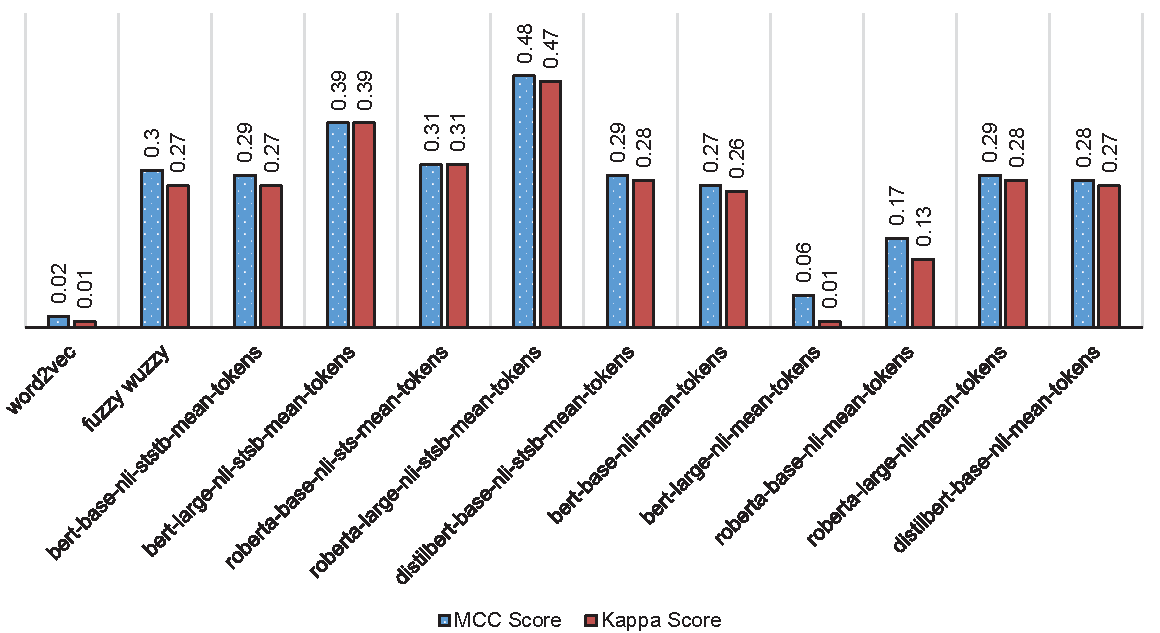
\includegraphics[scale=0.83]{evaluation_final}
	\caption{Performance evaluation of various models using MCC and kappa ($\kappa$) scores.}
	\label{fig:evaluation}
\end{figure*}

\section{Discussion}
\label{discussion}
In text classification, production and use of a well annotated corpus for supervised and semi-supervised learning is of utmost importance. The same is also useful for evaluating the performance of unsupervised learning techniques. In the real world, the production and maintenance of these corpora is an expensive task, often requiring extensive human effort and conformance to ethical principles, which can restrict access to critical data for the researchers. While there are many factors, influencing this reality, one of the most critical is the perception and cognitive ability of an expert user to subjectively assign a label to an instance \cite{reidsma2008exploiting, velupillai2010towards}. Data validity is especially important in the domain of healthcare, where the acquisition, curation, and sharing processes are all encapsulated by the need to ensure correctness as well as privacy and security of the user. Consequently, the availability of healthcare data, its accuracy, and transparency are major concerns for most researchers associated with this domain \cite{Joshi2018}. It is not only important to access the data but also to understand how it was produced, the caveats associated with it, and any assumptions made during or after its acquisition.  
In the case of our annotated dataset, the instances have been labeled by four human experts (two medical practitioners and two computer science graduates), using their subjective knowledge. One example of this subjective classification, is evident in the raw form of the data instances labeled by ``Annotator3''. According to ``Annotator3'' the relationship between the term ``AdmissionId'' and ``ClinicalHistory'' is parent-child. While the selection of this label can be debated from a subjective view point, changing or removing it or any other label, from the (objective) view point of the computing methodology would be incorrect\cite{pavlick2019inherent}. As a result, the annotations were kept anonymous so as not to induce any bias. Thus, the complete annotated data in its original form became the basis of our threshold selection and model evaluation methodology. A mode based voting mechanism was then used to resolve the differences between the annotators. The consolidated true dataset was then formed based on the agreed upon label by atleast 3 annotators. As pointed out in \cite{reidsma2008exploiting}, the net effect of such a voting mechanism is an increase in the precision of the machine learning classifiers in lieu of, their accuracy. As shown in the results and discussed further on, due to the bias nature of our dataset, accuracy measure is replaced by MCC. The lower scores of agreement between the (annotated data) true labels and predicted labels, have thus been evaluated in a contextual and relative manner.

Throughout this research work, the choice of performance metrics used for threshold selection and model evaluations are also driven by the dataset's nature. Even before annotation, the dataset is bias in favour of unrelated attributes. As established by the human experts and the machine learning model, for 254 attributes involved in 40698 possible pairs only a little over 300 similar instances are found. In these circumstances performance metrics, such as accuracy, precision, and recall are meaningless. These metrics are unable to account for the imbalanced datasets and provide an incorrect view of the classifier's accuracy. Instead metrics such as $F_1$, MCC, and $\kappa$ can provide a true picture of the classifier's accuracy. These metrics are also well suited for evaluating multi-class classifiers, using one vs all or one vs one binarizations of the dataset, as well as consolidating the results into a single measure. In our experimentation, we also evaluated the Area Under the Receiver Operating Characteristic (AUROC) curve and Area Under the Precision Recall (AUPR) curve, as a threshold selection metric. These graphs are well suited for independent classes as shown by \cite{espindola2005extending}. Additionally, in our case it is important to maximize the identification of similar attribute pairs ($class_1$), followed by related ones ($class_{0.5}$) and finally the unrelated ones($class_0$). AUROC and AUPR were thus replaced with our current approach for threshold selection. The benefit of using this kind of dependent classification is its usefulness in practice to identify a small set of similar attribute pairs, which can be used to establish positive results.

\section{Conclusion}
\label{conclusion}
Healthcare information systems are slowly moving towards a standardized approach, whereby the storage, exchange, and usage of health data, information, and knowledge is becoming interoperable. However, research and development of ubiquitous health management systems, still require manual interventions by human experts. These approaches require costly resource allocations, which are not possible for small and medium scaled healthcare service providers. In order to provide data interoperability services to these providers, and automating the process of generating maps between HMIS schema, which can match and transform patient data from a source provider to a target one, it is important to utilize state-of-the-art NLP techniques. Using transformer based pre-trained BERT models, we show the applicability of these techniques on creating the, as yet non-validated, schema maps. As a result, human effort can now focus on validating and verifying the schema maps, which can greatly accelerate the application of healthcare data interoperability, and provide a cohesive ecosystem for ubiquitous healthcare service delivery.
In future, we shall look towards developing a mechanism for schema map storage and evolution, along with expert validation to finally close this loop. We shall also work on re-training some of the existing pre-trained models, to improve the performance of schema map creation.

\section*{Acknowledgment}
This research was supported by ITRC(Information Technology Research Center) support program(IITP-2017-0-01629), Grand Information Technology Research Center support program(IITP-2021-2020-0-01489), and IITP-2017-0-00655 supervised by IITP(Institute of Information \& communications Technology Planning \& Evaluation), and National Research Foundation of Korea(NRF) NRF-2019R1A2C2090504 funded by the Korea government(MSIT).

\begin{thebibliography}{10}
	
	\bibitem{geraci1991ieee}
	Anne Geraci, Freny Katki, Louise McMonegal, Bennett Meyer, John Lane, Paul
	Wilson, Jane Radatz, Mary Yee, Hugh Porteous, and Fredrick Springsteel.
	\newblock {\em IEEE standard computer dictionary: Compilation of IEEE standard
		computer glossaries}.
	\newblock IEEE Press, 1991.
	
	\bibitem{Himss_url2013}
	{Healthcare Information and Management Systems Society}.
	\newblock {Definition of Interoperability}, 2013.
	
	\bibitem{khan2013process}
	Wajahat~Ali Khan, Maqbool Hussain, Khalid Latif, Muhammad Afzal, Farooq Ahmad,
	and Sungyoung Lee.
	\newblock Process interoperability in healthcare systems with dynamic semantic
	web services.
	\newblock {\em Computing}, 95(9):837--862, 2013.
	
	\bibitem{ali2017multi}
	Taqdir Ali, Maqbool Hussain, Wajahat~Ali Khan, Muhammad Afzal, Jamil Hussain,
	Rahman Ali, Waseem Hassan, Arif Jamshed, Byeong~Ho Kang, and Sungyoung Lee.
	\newblock Multi-model-based interactive authoring environment for creating
	shareable medical knowledge.
	\newblock {\em Computer Methods and Programs in Biomedicine}, 150:41--72, 2017.
	
	\bibitem{snomedct_url}
	{SNOMED Clinical Terminologies}.
	
	\bibitem{loinc}
	{LOINC}.
	
	\bibitem{mohammed2010ubiquitous}
	Sabah Mohammed and Jinan Fiaidhi.
	\newblock {\em Ubiquitous Health and Medical Informatics: The Ubiquity 2.0
		Trend and Beyond: The Ubiquity 2.0 Trend and Beyond}.
	\newblock IGI Global, 2010.
	
	\bibitem{CIMI2015}
	David Johnson.
	\newblock {Clinical Information Modeling Initiative (CIMI)}.
	\newblock Accessed:2021-06-05.
	
	\bibitem{Satti2020}
	Fahad~Ahmed Satti, Taqdir Ali, Jamil Hussain, Wajahat~Ali Khan, Asad~Masood
	Khattak, and Sungyoung Lee.
	\newblock {Ubiquitous Health Profile (UHPr): a big data curation platform for
		supporting health data interoperability}.
	\newblock {\em Computing}, 2020.
	
	\bibitem{althubaiti2020combining}
	Sara Althubaiti, {\c{S}}enay Kafkas, Marwa Abdelhakim, and Robert Hoehndorf.
	\newblock Combining lexical and context features for automatic ontology
	extension.
	\newblock {\em Journal of biomedical semantics}, 11(1):1--13, 2020.
	
	\bibitem{nozaki2019semantic}
	Kenji Nozaki, Teruhisa Hochin, and Hiroki Nomiya.
	\newblock Semantic schema matching for string attribute with word vectors.
	\newblock In {\em 2019 6th International Conference on Computational
		Science/Intelligence and Applied Informatics (CSII)}, pages 25--30. IEEE,
	2019.
	
	\bibitem{yousfi2020xmatcher}
	Aola Yousfi, Moulay~Hafid El~Yazidi, and Ahmed Zellou.
	\newblock xmatcher: Matching extensible markup language schemas using
	semantic-based techniques.
	\newblock {\em International Journal of Advanced Computer Science and
		Applications}, 11(8):655--665, 2020.
	
	\bibitem{bulygin2018combining}
	Lev Bulygin.
	\newblock Combining lexical and semantic similarity measures with machine
	learning approach for ontology and schema matching problem.
	\newblock In {\em Proceedings of the XX International Conference “Data
		Analytics and Management in Data Intensive Domains”(DAMDID/RCDL’2018)},
	pages 245--249, 2018.
	
	\bibitem{martono2017review}
	Galih~Hendro Martono and SN~Azhari.
	\newblock Review implementation of linguistic approach in schema matching.
	\newblock {\em International Journal of Advances in Intelligent Informatics},
	3(1):1--9, 2017.
	
	\bibitem{alwan2017survey}
	Ali~A Alwan, Azlin Nordin, Mogahed Alzeber, and Abedallah~Zaid Abualkishik.
	\newblock A survey of schema matching research using database schemas and
	instances.
	\newblock {\em International Journal of Advanced Computer Science and
		Applications}, 8(10), 2017.
	
	\bibitem{kersloot2020natural}
	Martijn~G Kersloot, Florentien~JP van Putten, Ameen Abu-Hanna, Ronald Cornet,
	and Derk~L Arts.
	\newblock Natural language processing algorithms for mapping clinical text
	fragments onto ontology concepts: a systematic review and recommendations for
	future studies.
	\newblock {\em Journal of biomedical semantics}, 11(1):1--21, 2020.
	
	\bibitem{xu2003discovering}
	Li~Xu and David~W Embley.
	\newblock Discovering direct and indirect matches for schema elements.
	\newblock In {\em Eighth International Conference on Database Systems for
		Advanced Applications, 2003.(DASFAA 2003). Proceedings.}, pages 39--46. IEEE,
	2003.
	
	\bibitem{zhu2018exploring}
	Xunjie Zhu, Tingfeng Li, and Gerard De~Melo.
	\newblock Exploring semantic properties of sentence embeddings.
	\newblock In {\em Proceedings of the 56th Annual Meeting of the Association for
		Computational Linguistics (Volume 2: Short Papers)}, pages 632--637, 2018.
	
	\bibitem{kartoun2016methodology}
	Uri Kartoun.
	\newblock A methodology to generate virtual patient repositories.
	\newblock {\em arXiv preprint arXiv:1608.00570}, 2016.
	
	\bibitem{pan2016design}
	Lijun Pan, Xiaoting Fu, Fangfang Cai, Yu~Meng, and Changjiang Zhang.
	\newblock Design a novel electronic medical record system for regional clinics
	and health centers in china.
	\newblock In {\em 2016 2nd IEEE International Conference on Computer and
		Communications (ICCC)}, pages 38--41. IEEE, 2016.
	
	\bibitem{inokuchi2007medtakmi}
	Akihiro Inokuchi, Koichi Takeda, Noriko Inaoka, and Fumihiko Wakao.
	\newblock Medtakmi-cdi: interactive knowledge discovery for clinical decision
	intelligence.
	\newblock {\em IBM Systems Journal}, 46(1):115--133, 2007.
	
	\bibitem{ali2017reconciliation}
	Taqdir Ali and Sungyoung Lee.
	\newblock Reconciliation of snomed ct and domain clinical model for
	interoperable medical knowledge creation.
	\newblock In {\em 2017 39th Annual International Conference of the IEEE
		Engineering in Medicine and Biology Society (EMBC)}, pages 2654--2657. IEEE,
	2017.
	
	\bibitem{reimers-2019-sentence-bert}
	Nils Reimers and Iryna Gurevych.
	\newblock Sentence-bert: Sentence embeddings using siamese bert-networks.
	\newblock In {\em Proceedings of the 2019 Conference on Empirical Methods in
		Natural Language Processing}. Association for Computational Linguistics, 11
	2019.
	
	\bibitem{chicco2020advantages}
	Davide Chicco and Giuseppe Jurman.
	\newblock The advantages of the matthews correlation coefficient (mcc) over f1
	score and accuracy in binary classification evaluation.
	\newblock {\em BMC genomics}, 21(1):1--13, 2020.
	
	\bibitem{gwet2014handbook}
	Kilem~L Gwet.
	\newblock {\em Handbook of inter-rater reliability: The definitive guide to
		measuring the extent of agreement among raters}.
	\newblock Advanced Analytics, LLC, 2014.
	
	\bibitem{FuzzyWuzzy}
	{Adam Cohen}.
	\newblock Fuzzywuzzy: Fuzzy string matching in python, Jul 8th, 2011.
	
	\bibitem{mchugh2012interrater}
	Mary~L McHugh.
	\newblock Interrater reliability: the kappa statistic.
	\newblock {\em Biochemia medica}, 22(3):276--282, 2012.
	
	\bibitem{reidsma2008exploiting}
	Dennis Reidsma and Rieks op~den Akker.
	\newblock Exploiting ‘subjective’annotations.
	\newblock In {\em Coling 2008: Proceedings of the workshop on Human Judgements
		in Computational Linguistics}, pages 8--16, 2008.
	
	\bibitem{velupillai2010towards}
	Sumithra Velupillai.
	\newblock Towards a better understanding of uncertainties and speculations in
	swedish clinical text--analysis of an initial annotation trial.
	\newblock In {\em Proceedings of the Workshop on Negation and Speculation in
		Natural Language Processing}, pages 14--22, 2010.
	
	\bibitem{Joshi2018}
	Mohit Joshi and Payal Bhardwaj.
	\newblock {Impact of data transparency: Scientific publications}.
	\newblock {\em Perspectives in Clinical Research}, 9(1):31--36, 2018.
	
	\bibitem{pavlick2019inherent}
	Ellie Pavlick and Tom Kwiatkowski.
	\newblock Inherent disagreements in human textual inferences.
	\newblock {\em Transactions of the Association for Computational Linguistics},
	7:677--694, 2019.
	
	\bibitem{espindola2005extending}
	Rog{\'e}rio~P Esp{\'\i}ndola and Nelson~FF Ebecken.
	\newblock On extending f-measure and g-mean metrics to multi-class problems.
	\newblock {\em WIT Transactions on Information and Communication Technologies},
	35, 2005.
	
	\bibitem{moll2020oncology}
	Jonas Moll and {\AA}sa Cajander.
	\newblock Oncology health-care professionals’ perceived effects of patient
	accessible electronic health records 6 years after launch: a survey study at
	a major university hospital in sweden.
	\newblock {\em Health informatics journal}, 26(2):1392--1403, 2020.
	
\end{thebibliography}

% orcid: 0000-0002-9883-3355
\begin{IEEEbiography}[{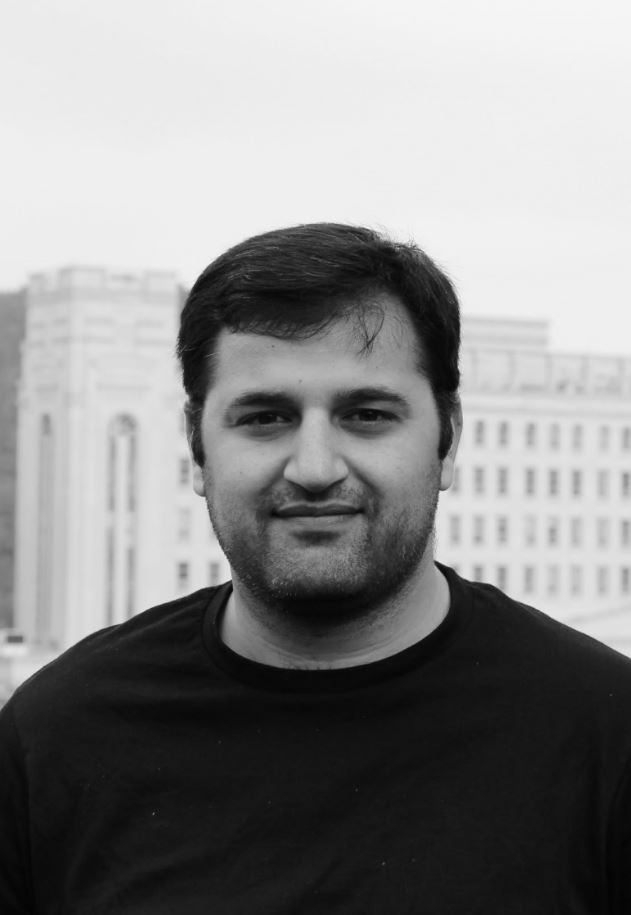
\includegraphics[width=1in,height=1.25in,clip,keepaspectratio]{fahad.jpg}}]{Fahad Ahmed Satti} is currently pursuing Ph.D. in Computer Engineering from Kyung Hee University, South Korea. He completed his MS in Computer Science from University of Trento, Italy in 2014. His primary research interest is directed towards providing a technical solution to resolve the lack of interoperability in information systems. In general, he is interested in domains of semantic matching, stream reasoning, knowledge extraction, and machine learning.
\end{IEEEbiography}
% orcid: 0000-0003-4494-1593
\begin{IEEEbiography}[{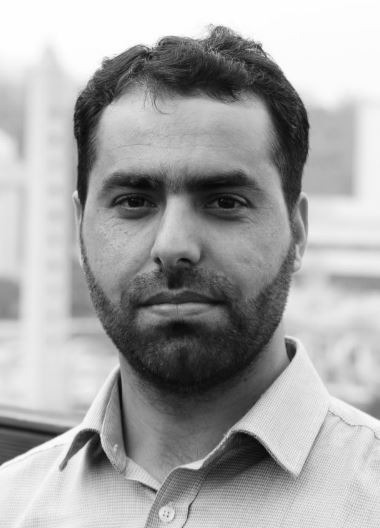
\includegraphics[width=1in,height=1.25in,clip,keepaspectratio]{musarrat.jpg}}]{Musarrat Hussain} is a Ph.D. candidate in the Ubiquitous Computing Laboratory, Kyung Hee University, 	South Korea. He has completed his MS software Engineering in 2015 from National University of Science 	and Technology (NUST) Pakistan. His research interests include clinical text mining, knowledge 	extraction and representation, and machine learning.
\end{IEEEbiography}
% orcid: 0000-0003-3862-8787
\begin{IEEEbiography}[{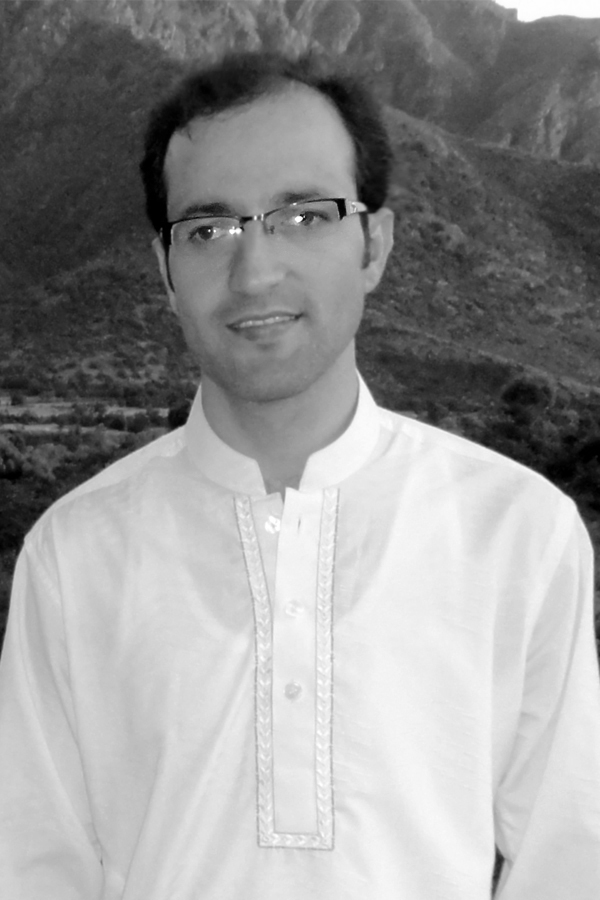
\includegraphics[width=1in,height=1.25in,clip,keepaspectratio]{jamil.jpg}}]{Jamil Hussain} received the Ph.D. degree from the Department of Computer Engineering, Kyung Hee University, South Korea in 2019. He worked as a postdoctoral researcher in the Ubiquitous Computing Laboratory, Kyung Hee University, South Korea, from Sep 2019 to Feb 2021. He is currently an Assistant Professor at Sejong University, South Korea. He has professional experience of over 7 years in the software industry, working on user experience design and development on various projects. His research interest includes user experience design, artificial intelligence, and information extraction from textual data.
\end{IEEEbiography}
% orcid: 0000-0001-8450-6946
\begin{IEEEbiography}[{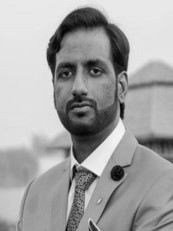
\includegraphics[width=1in,height=1.25in,clip,keepaspectratio]{imran.jpg}}]{Syed Imran Ali} received the BS degree in Computer Science from IQRA University, Islamabad in 2008 and MS degree in Computer Science From National University of Computer and Emerging Sciences (NUCES) in 2012. He has taught in NUCES as an adjunct faculty. He is currently pursuing Ph.D. degree from Department of Computer Science and Engineering, Kyung Hee University, South Korea. His area of interests include machine learning, health analytics and data-driven systems.
\end{IEEEbiography}
% orcid: 0000-0001-8450-6946
\begin{IEEEbiography}[{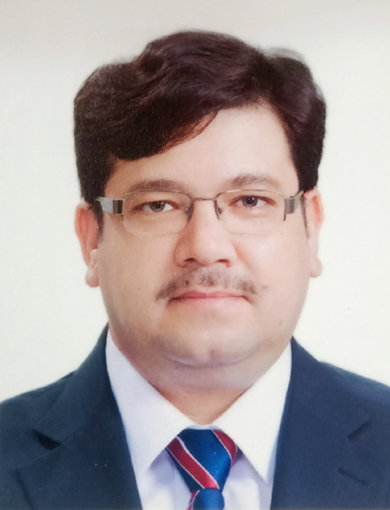
\includegraphics[width=1in,height=1.25in,clip,keepaspectratio]{taqdir.jpg}}]{Taqdir Ali} received the Ph.D. degree from the Department of Computer Engineering, Kyung Hee University, South Korea in 2019. He is currently working as a postdoctoral researcher in the Ubiquitous Computing Laboratory, Kyung Hee University, South Korea. From 2006 to 2011, he was a Senior Software Engineer, a System Analyst, and a Researcher in a reputable software house. His current research includes knowledge acquisition for clinical decision support systems, applications of machine learning, text processing, and e-health standardization.
\end{IEEEbiography}
% orcid: 0000-0002-8920-4231
\begin{IEEEbiography}[{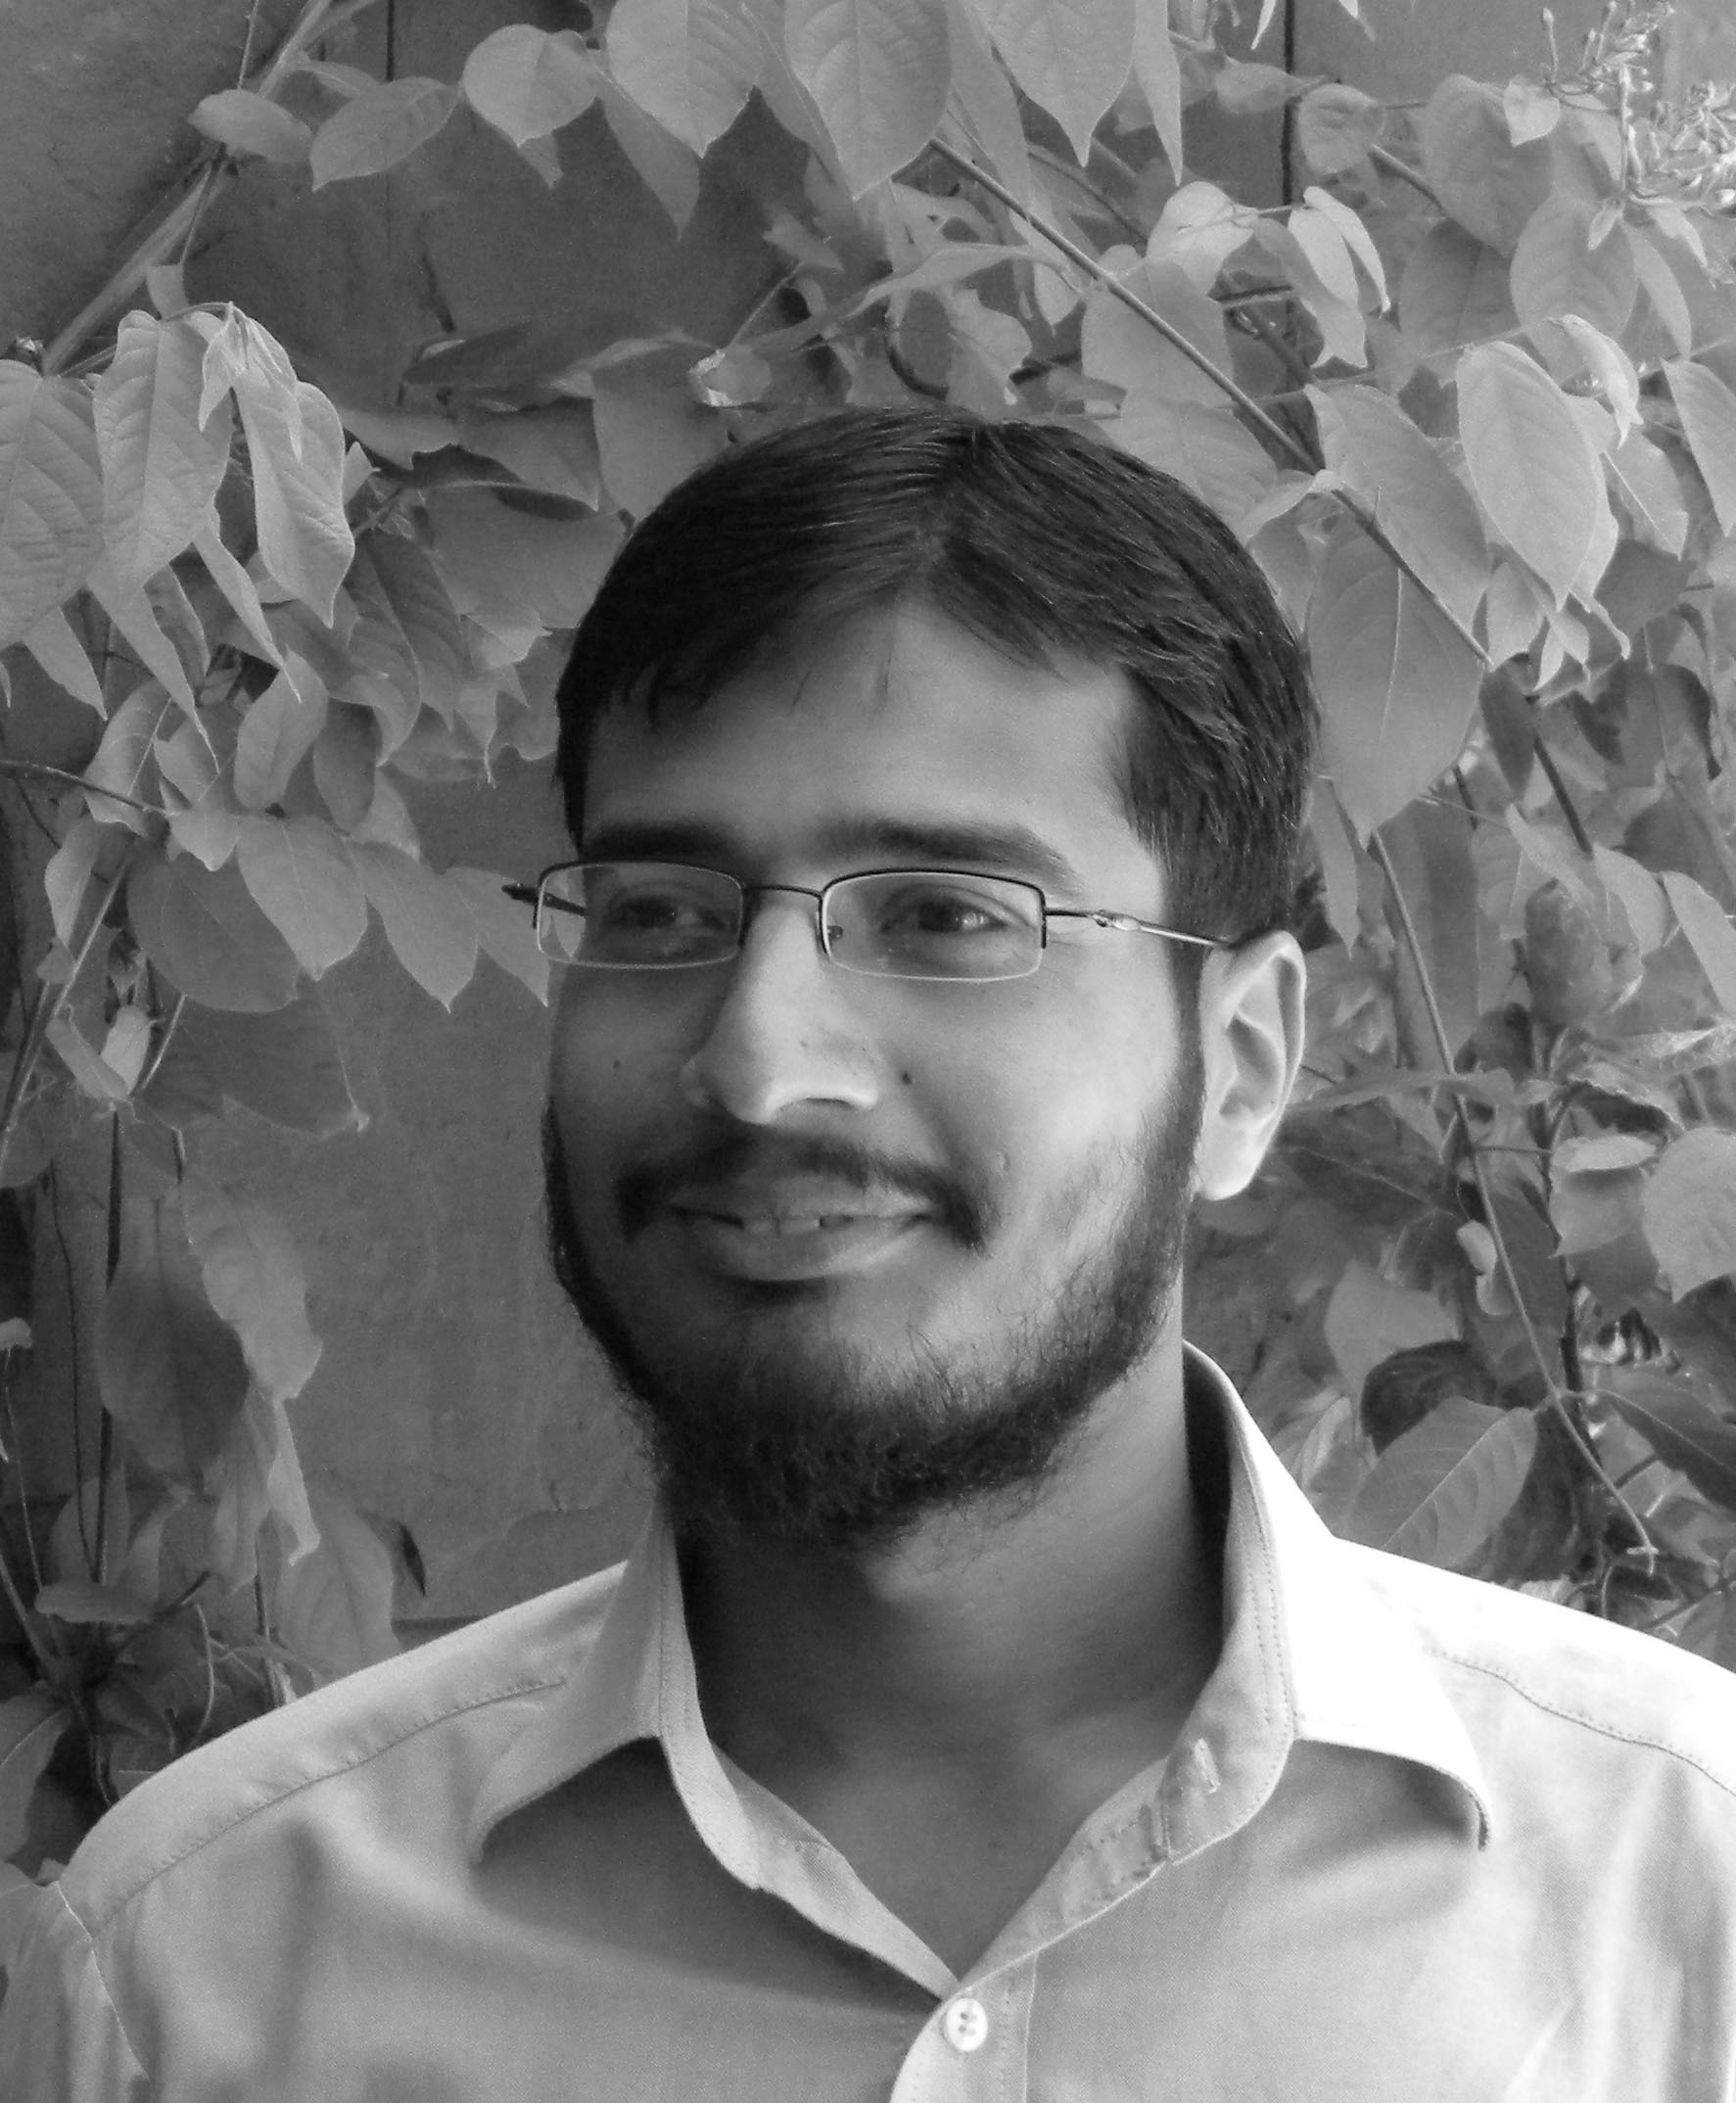
\includegraphics[width=1in,height=1.25in,clip,keepaspectratio]{bilal.jpg}}]{Hafiz Syed Muhammad Bilal}  received the M.S. degree in computer science from National University of Sciences and Technology, Pakistan,in 2008. He is currently pursuing the Ph.D. degree in computer science and engineering at Kyung Hee University, South Korea. He has working experience of more than three years in data science and open source development and is actively involved in developing big data ecosystem for academic and health care. His research interests include behavior quantification \& assessment, machine learning, and behavior modeling \& adaptation.
\end{IEEEbiography}
\begin{IEEEbiography}[{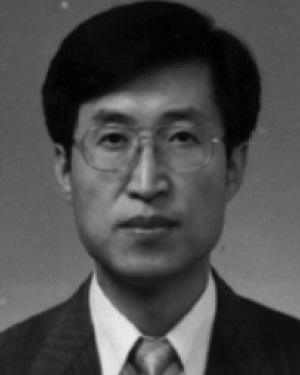
\includegraphics[width=1in,height=1.25in,clip,keepaspectratio]{prof_tcc.jpg}}]{TaeChoong Chung}  received his B.S. degree in Electronic Engineering from Seoul National University, Republic of Korea, in 1980, and his M.S. and Ph.D. degrees in Computer Science from KAIST, Republic of Korea, in 1982 and 1987, respectively. Since 1988, he has been with the Department of Computer Science and Engineering, Kyung Hee University, Republic of Korea, where he is now a Professor. His research interests include machine learning, meta search, and robotics.
\end{IEEEbiography}
% orcid: 0000-0002-5962-1587
\begin{IEEEbiography}[{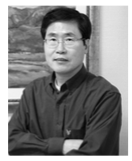
\includegraphics[width=1in,height=1.25in,clip,keepaspectratio]{prof_sylee.png}}]{Sungyoung Lee} received the B.S.degree from Korea University, Seoul, South Korea,and the M.S. and Ph.D. degrees in computer science from the Illinois Institute of Technology,Chicago, IL, USA, in 1987 and 1991, respectively.He was an Assistant Professor with the Department of Computer Science, Governors State University, University Park, IL, USA, from 1992 to 1993. He has been a Professor with the Department of Computer Engineering, Kyung Hee University,South Korea, since 1993, where he has been the Director of the Neo Medical ubiquitous-Life Care Information Technology Research Center since 2006.He is currently the Founding Director of the Ubiquitous Computing Laboratory. His current research interests include ubiquitous computing and applications, wireless ad hoc and sensor networks, context-aware middle-ware, sensor operating systems, real-time systems and embedded systems,and activity and emotion recognition. He is a member of ACM.
\end{IEEEbiography}

\EOD

\end{document}
